\section{Introduction}
{\it Movement primitives}, mathematical models that encode trajectories {\it offline}, enable rapid {\it online} trajectory generation~\cite{park2008movement, paraschos2013probabilistic, khansari2011learning, noseworthy2020task, lee2023equivariant, lee2024mmp++}, where data are typically collected from human demonstrations. They avoid the need for time-consuming online motion planning that reduces the system's reactivity, allowing fast adaptation to changes in environments. 

In this paper, we adopt the view that effective primitive models should satisfy two key properties. First, they should encode a diverse set of trajectories for a given task to enhance adaptability, ensuring that if some trajectories become unexecutable, such as being blocked by unforeseen obstacles, feasible alternatives remain available. Second, they should be capable of generating motions conditioned on task-defining parameters, such as vision data describing the environment or language commands reflecting user intent, ensuring applicability across a wide range of tasks.

Learning these primitives poses two main challenges.
First, obtaining a sufficiently large dataset of human demonstrations is challenging, often leading to limited data availability. This difficulty is amplified by the need to collect data for each specific task parameter, further increasing data demands.
Second, trajectory data is inherently high-dimensional, particularly for long-horizon motions. When expressed as a sequence of configurations at discrete time steps, its dimensionality increases linearly with the number of time steps.


Leveraging a low-dimensional manifold structure can be an effective solution. Assuming the set of demonstration trajectories lies on a lower-dimensional manifold embedded in the trajectory space (the manifold hypothesis), recent works have focused on identifying this manifold to reduce data dimensionality and address both challenges~\cite{noseworthy2020task, lee2023equivariant}. Task-conditioned variational autoencoders (TCVAE)~\cite{noseworthy2020task} and motion manifold primitives (MMP)~\cite{lee2023equivariant} employ conditional autoencoder architectures, demonstrating promising results for task-conditioned, diverse, high-dimensional trajectory generation.

\begin{figure}[!t]
    \centering
    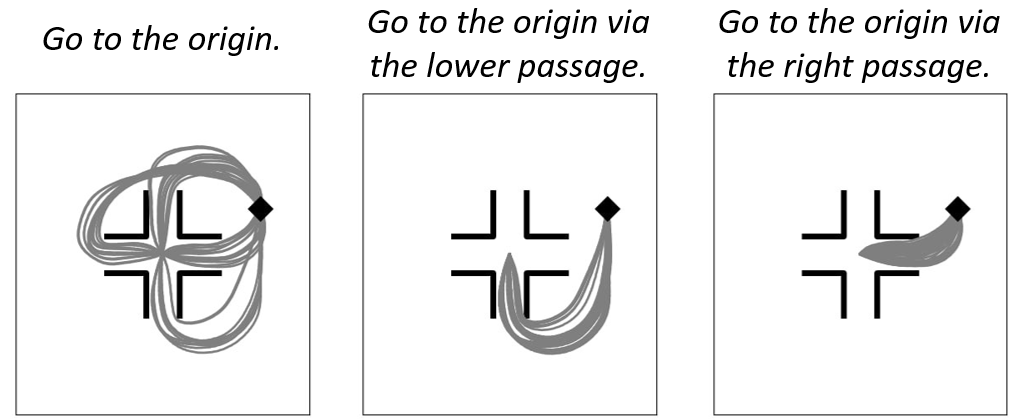
\includegraphics[width=\linewidth]{tabs/figures/ral_intro_2d.png}
        \caption{An illustrative example of a language-guided navigation scenario with complex task-motion dependencies: The motion distribution shifts dramatically -- for instance, in the number of modalities -- when the task parameter (in this case, a language command) changes.}
    \label{fig:example}
    \vspace{-10pt}
\end{figure}

However, existing manifold-based models fail to capture the {\it complex} task dependencies of motion distributions, where ``complex dependencies'' refer to cases in which the motion distribution undergoes dramatic shifts (e.g., changes in the number of modalities or the volume of support) as the task parameter varies.
For example, consider the navigation scenario shown in Fig.~\ref{fig:example}, where the task parameter is specified by a language command. If the command is ``Go to the origin'', the robot can select any of the four available passages. However, if the command changes to ``Go to the origin via the lower passage'', the robot must exclusively take the lower passage. This change drastically alters the motion distribution, reducing the number of modalities. As we demonstrate later in our experiments, existing models fail in these scenarios. The fundamental reason for these failures is their reliance on conditional autoencoder architectures with a shared latent prior distribution, as we detail in Section~\ref{sec:limit}.

In this paper, we propose Motion Manifold Flow Primitives (MMFP), a framework that decouples the training of the motion manifold and task-conditioned distributions, effectively capturing complex task-motion dependencies. Our approach leverages flow matching models~\cite{lipman2022flow,chen2023riemannian}, state-of-the-art conditional deep generative models capable of effectively capturing complex conditional distributions, in the latent coordinate space of the learned motion manifold. As a result, MMFP simultaneously addresses the challenges of limited datasets, high dimensionality, and complex task-motion dependencies, and significantly outperforms existing manifold-based models.

It is instructive to highlight the differences between recent learning-from-demonstration methods based on diffusion and flow matching models -- such as diffusion policies~\cite{chi2023diffusion,ze20243d} and flow matching policies~\cite{braun2024riemannian,chisari2024learning} -- and our proposed MMFP. The key distinction lies in whether the low-dimensional manifold structure is explicitly utilized. These existing methods focus on generating relatively low-dimensional \emph{local} trajectories for policy learning, whereas our aim is to produce \emph{global}, high-dimensional trajectories for motion planning, requiring dimensionality reduction. As we show in our experiments, simply training diffusion or flow matching models without manifold learning fails to generate valid global trajectories.

We provide case studies on language-guided trajectory generation, where each demonstration trajectory is paired with multiple hierarchical text descriptions.  
This setup introduces many-to-many mappings between text and motion, leading to complex text dependencies in the motion distributions.  
Two text-based trajectory generation tasks are considered: (i) SE(3) trajectory generation for a bottle in a pouring task and (ii) 7-DoF robot arm trajectory generation for a waving task. Notably, with only 10 and 30 demonstration trajectories for each task, respectively, MMFP demonstrates excellent performance.  
In contrast, diffusion and flow-based models trained directly in the high-dimensional trajectory space~\cite{ho2020denoising, lipman2022flow, chen2023riemannian} and existing motion manifold-based methods~\cite{noseworthy2020task, lee2023equivariant} fail to generate successful trajectories.